\documentclass[10pt,a4paper]{article}
\usepackage[utf8]{inputenc}
\usepackage[T1]{fontenc}
\usepackage[spanish,es-noshorthands,es-tabla]{babel}
\usepackage{amsmath}
\usepackage{graphicx}
\usepackage{booktabs}
\usepackage{float}
\usepackage[margin=1.8cm]{geometry}
\usepackage[font=small]{caption}
\usepackage{titlesec}
\titlespacing*{\section}{0pt}{8pt}{3pt}
\setlength{\parskip}{3pt}
\setlength{\parindent}{0pt}
\pagestyle{empty}

\begin{document}

\begin{center}
  {\Large\bfseries Simulación del control de J1 (base) y J3 (codo)}\\[2pt]
  {\small Brazo del recolector de frutas, 4 de octubre de 2026}
\end{center}

\section{La idea}
Cada articulación se controla con dos lazos, uno dentro del otro: el de \textbf{posición} compara el ángulo pedido con
el medido y decide a qué velocidad moverse, y el de \textbf{velocidad} decide cuánta potencia (duty $u$, en \%) darle
al motor (figura~\ref{fig:diagrama}). \textbf{Simular} es calcular en la computadora cómo se va a mover, con una
ecuación del motor (la \emph{planta}) y el mismo control de la placa, y después compararlo con lo que pasó de verdad.

\section{Las ecuaciones}
\textbf{Planta:} con un duty $u$ la velocidad $\omega$ tiende a $K(u-u_c)$ y tarda unos $\tau$ segundos en llegar;
$u_c$ es la zona muerta (con menos duty, el motor no se mueve).
\[
  \tau\,\frac{d\omega}{dt}=-\omega+K\,(u-u_c)\quad\Longrightarrow\quad G(s)=\frac{K}{\tau s+1}
\]
\textbf{Control de velocidad (PI):} una parte fija que vence la zona muerta, una proporcional al error y una que lo
acumula para que no quede diferencia al final.
\[
  u=u_{ff}+K_p\,e+K_i\!\int e\,dt,\quad e=\omega_{ref}-\omega
  \qquad\Longrightarrow\qquad
  \frac{\omega}{\omega_{ref}}=\frac{K\,(K_p s+K_i)}{\tau s^2+(1+K K_p)\,s+K K_i}
\]
\textbf{Control de posición (P):} pide $\omega_{ref}=K_{pp}(\theta_{ref}-\theta)$. Si el lazo de velocidad tarda
$\tau_v$ en responder, no se pasa del ángulo pedido mientras $K_{pp}\le 1/(4\tau_v)$:
\[
  \frac{\theta}{\theta_{ref}}=\frac{K_{pp}}{\tau_v s^2+s+K_{pp}}
\]

\section{Resultados}
{\small
\begin{tabular}{@{}p{3.6cm}p{6.3cm}p{6.6cm}@{}}
  \toprule
  & \textbf{J1 (base)} & \textbf{J3 (codo)} \\
  \midrule
  Planta & $G_1=\dfrac{1{,}90}{0{,}065\,s+1}$, zona muerta 17\,\% & $G_3=\dfrac{1{,}62}{0{,}053\,s+1}$, zona muerta
  $23{,}6+1{,}42\,\theta$\,\% subiendo (peso del antebrazo) y 3,2\,\% bajando \\[8pt]
  De dónde sale & pruebas del motor solo & ajustada con las pruebas guardadas (fig.~\ref{fig:j3id}) \\
  Ganancias & $K_p=0{,}549$, $K_i=4$, $K_{pp}=2$ & $K_p=0{,}35$, $K_i=5$, $K_{pp}=2$ \\[3pt]
  Lazo de velocidad & $\dfrac{1{,}90\,(0{,}549\,s+4)}{0{,}065\,s^2+2{,}04\,s+7{,}58}$ &
  $\dfrac{1{,}62\,(0{,}35\,s+5)}{0{,}053\,s^2+1{,}57\,s+8{,}1}$ \\[10pt]
  Lazo de posición & $\dfrac{2}{0{,}09\,s^2+s+2}$ (no se pasa si $K_{pp}\le 2{,}78$) &
  $\dfrac{2}{0{,}12\,s^2+s+2}$ (no se pasa si $K_{pp}\le 2{,}08$) \\[10pt]
  Llegada: placa / simulación & 1,71--1,77\,s / 1,64\,s (escalones de $\pm20^\circ$) &
  sube: 1,30 / 1,29\,s; baja a $-10^\circ$: \textbf{1,92 / 1,06\,s} ($\pm10^\circ$) \\
  Se pasa del objetivo & no / no & no / no \\
  Error final (placa) & $\le 0{,}30^\circ$ & $\le 0{,}29^\circ$ \\
  \bottomrule
\end{tabular}
}

\section{Conclusiones}
\begin{itemize}\setlength{\itemsep}{1pt}
  \item \textbf{J1:} un modelo simple del motor alcanza para diseñar el control; la placa llega solo 0,1\,s más tarde que
        la simulación por el juego de la correa (figuras~\ref{fig:j1v} y~\ref{fig:j1p}).
  \item \textbf{J3:} hubo que sumar al modelo el peso del antebrazo. Con eso la simulación acierta subiendo y confirma
        que $K_{pp}=2$ no se pasa del objetivo (figura~\ref{fig:j3p}). Bajando hacia $-10^\circ$ la placa tarda casi el
        doble: ahí el mecanismo se endurece y el modelo no lo tiene.
  \item En las dos articulaciones el control llega al ángulo pedido \textbf{sin pasarse} y con error menor a $0{,}3^\circ$.
\end{itemize}

\clearpage
\section{Figuras}

\begin{figure}[H]
  \centering
  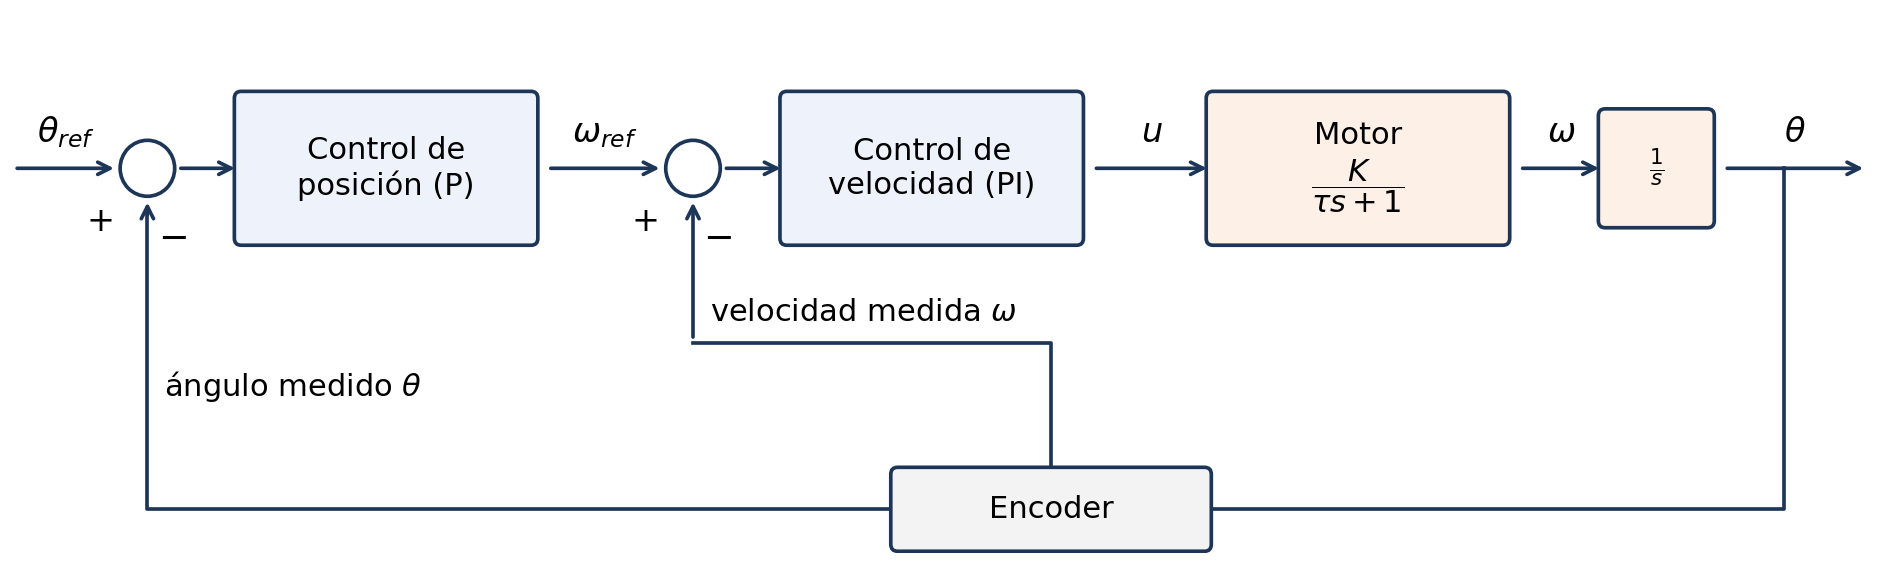
\includegraphics[width=\textwidth]{diagrama_control.png}
  \caption{Los dos lazos del control. El encoder mide el ángulo y, con él, la velocidad.}
  \label{fig:diagrama}
\end{figure}

\begin{figure}[H]
  \centering
  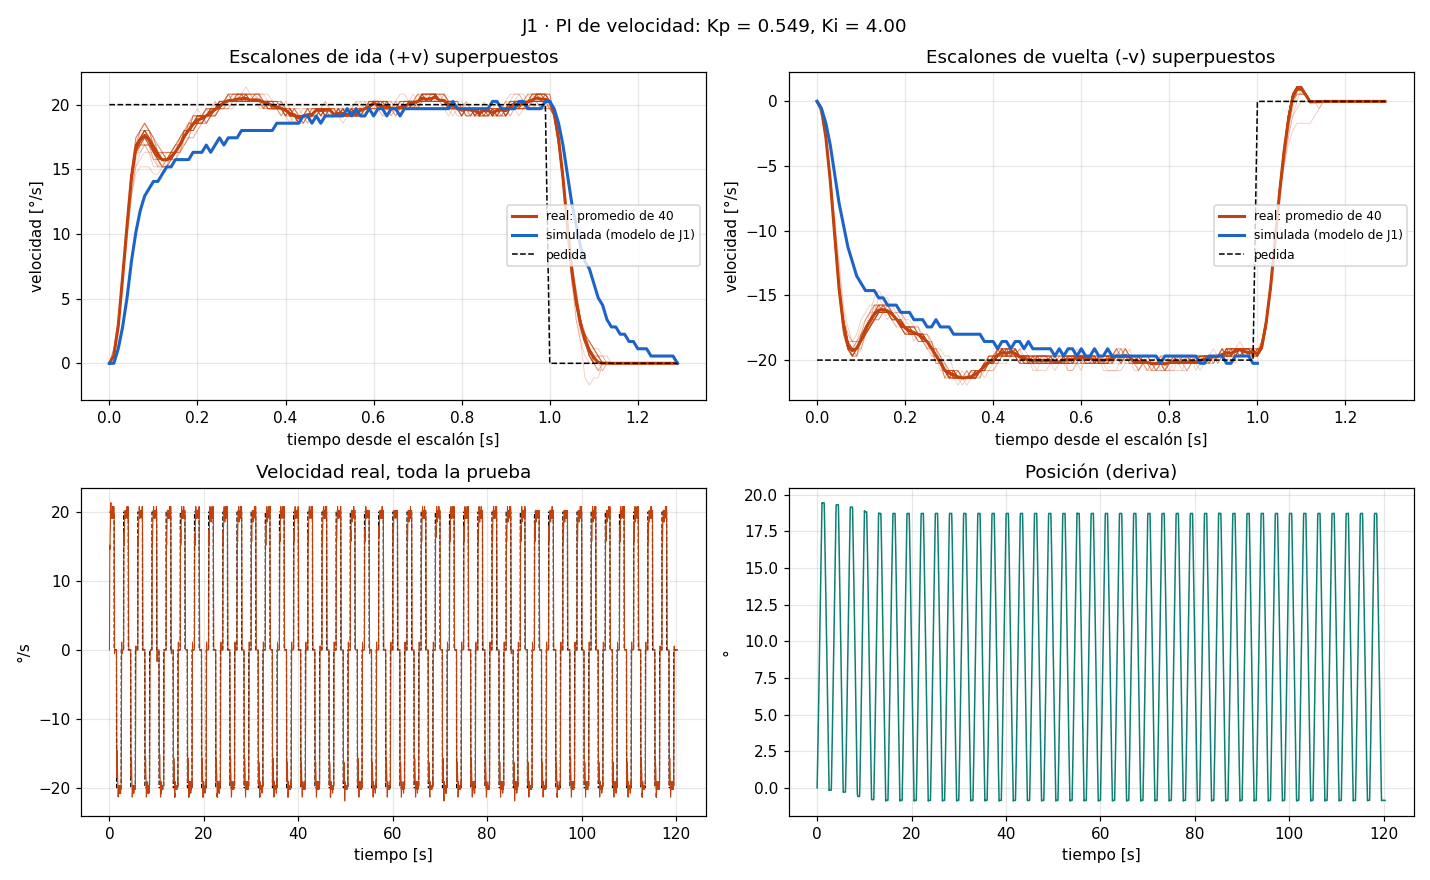
\includegraphics[width=\textwidth]{j1/j1_4_comparacion_velocidad_sim_vs_real.png}
  \caption{J1, velocidad: 40 escalones de $\pm 20\ ^\circ/s$ en la placa (rojo) y la simulación (azul).}
  \label{fig:j1v}
\end{figure}

\begin{figure}[H]
  \centering
  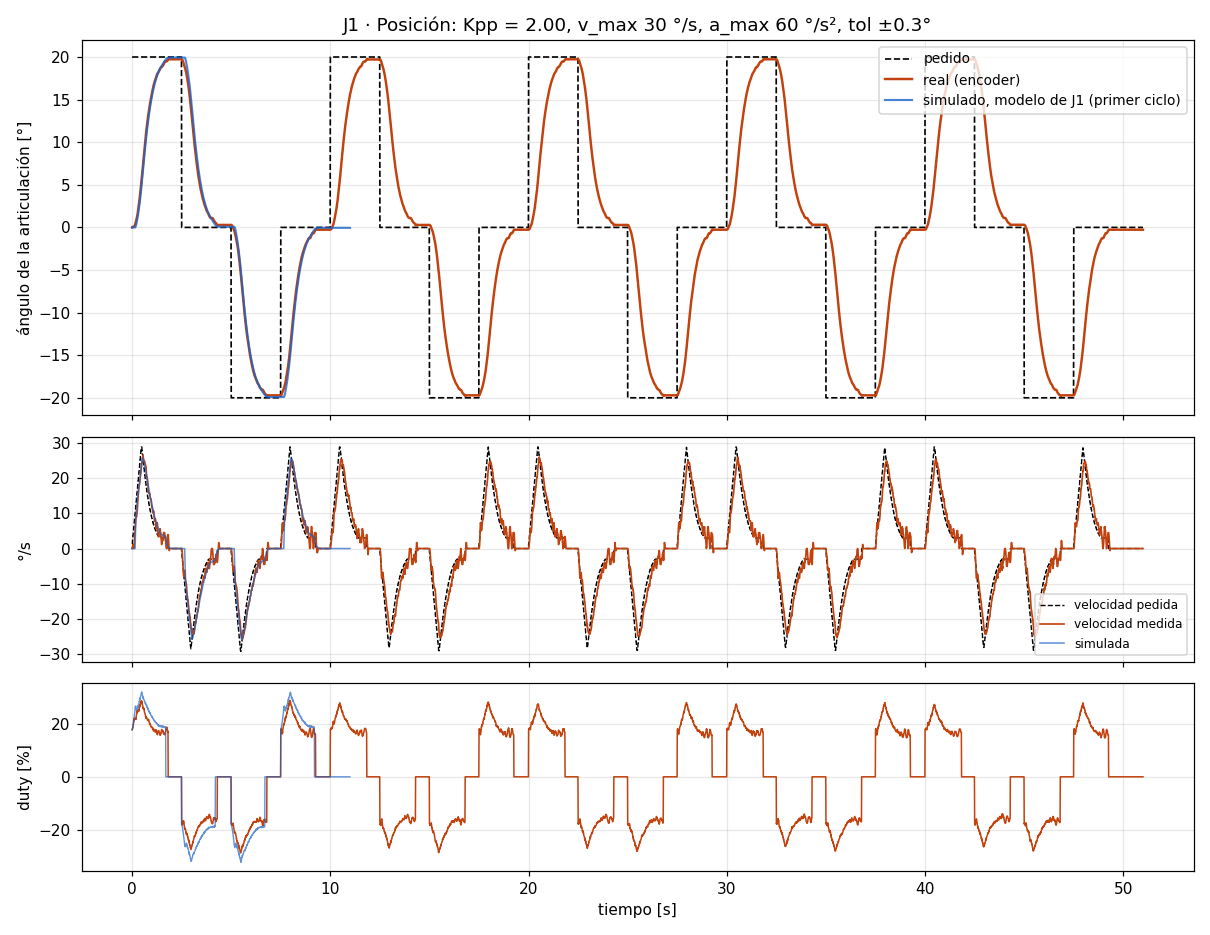
\includegraphics[width=0.85\textwidth]{j1/j1_5_comparacion_posicion_sim_vs_real.png}
  \caption{J1, posición: 20 escalones de $\pm 20^\circ$ en la placa (rojo) y la simulación (azul).}
  \label{fig:j1p}
\end{figure}

\begin{figure}[H]
  \centering
  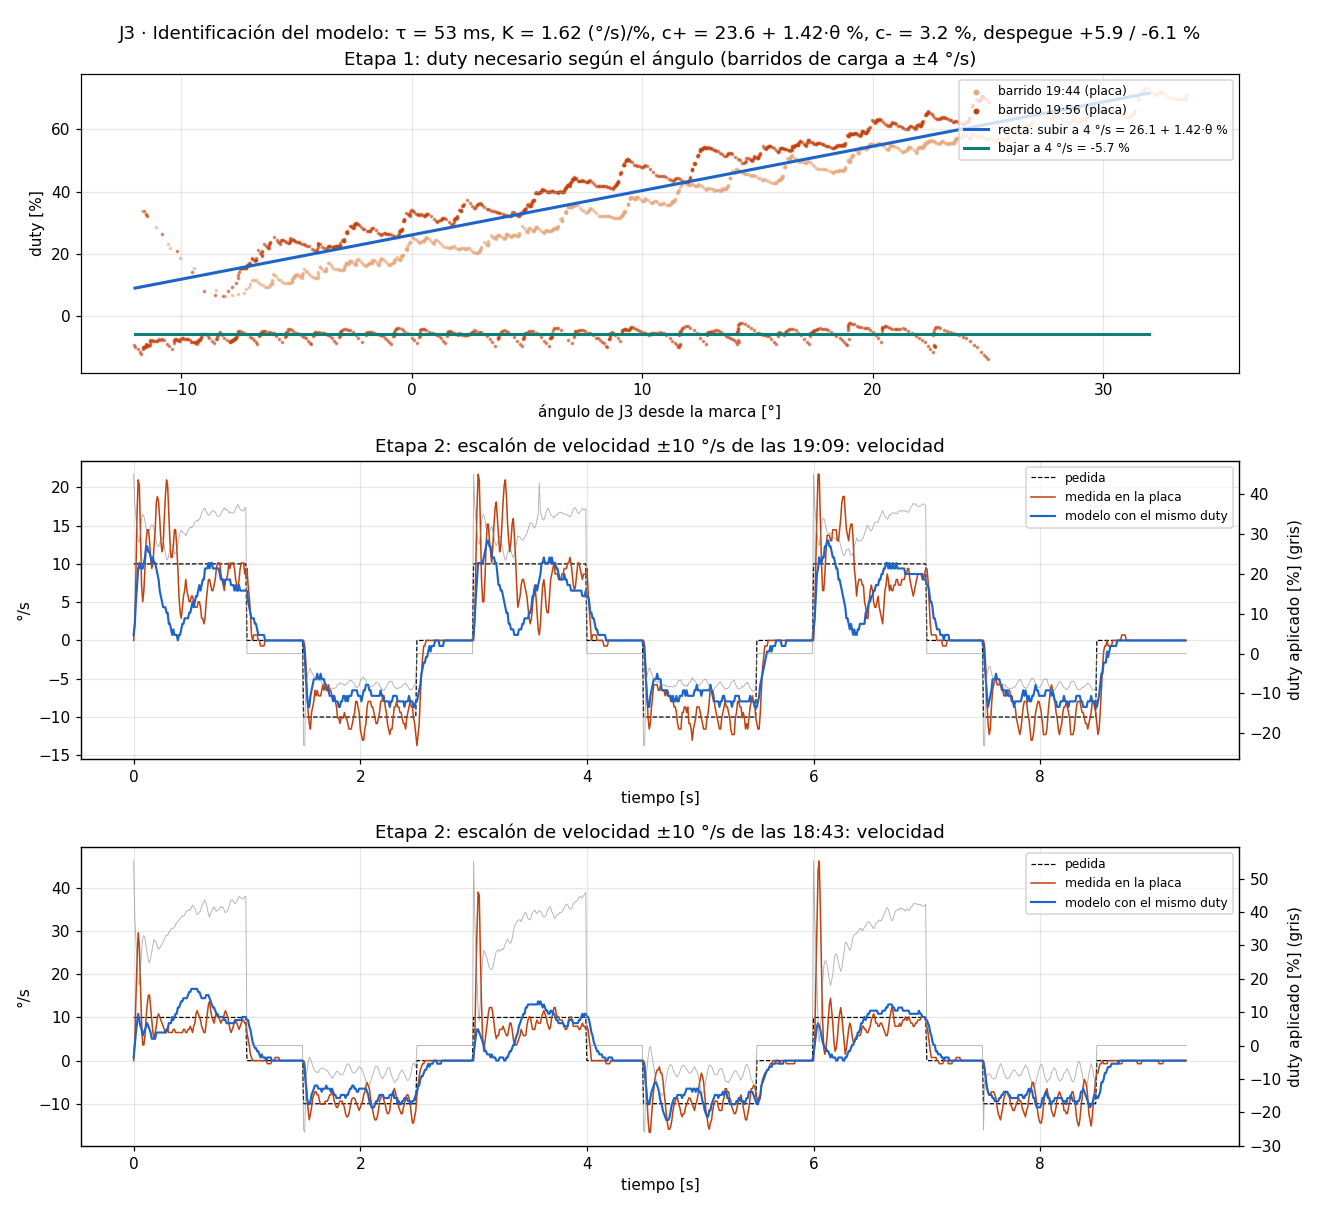
\includegraphics[width=0.85\textwidth]{j3/j3_1_identificacion_planta.png}
  \caption{J3, cómo se obtuvo el modelo: arriba, el duty que hace falta según el ángulo (crece al subir por el peso);
  abajo, la velocidad medida (rojo) y la del modelo con el mismo duty (azul).}
  \label{fig:j3id}
\end{figure}

\begin{figure}[H]
  \centering
  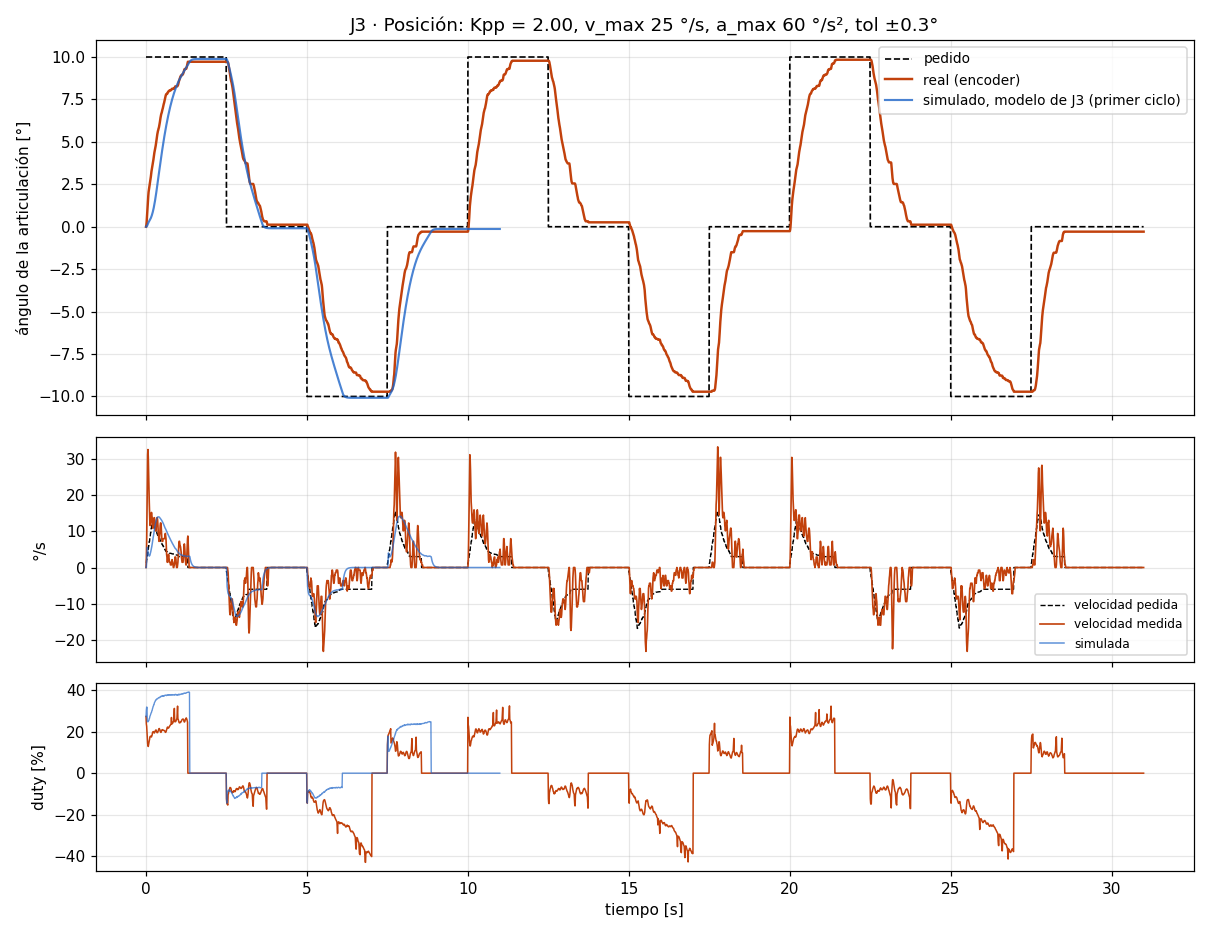
\includegraphics[width=0.85\textwidth]{j3/j3_7_comparacion_posicion_sim_vs_real_final.png}
  \caption{J3, posición: 12 escalones de $\pm 10^\circ$ en la placa (rojo) y la simulación (azul).}
  \label{fig:j3p}
\end{figure}

\end{document}
